\section{\uppercase{Deconstruction Application for surveyors}}
\label{sec:application}

\noindent Una decostruzione efficiente ed improntata al massimo riuso dei materiali, deve essere necessariamente supportata da una corretta metodologia che guidi l'utente verso una pianificazione e stima dei costi del processo. Verr\`a presentata di seguito la metodologia individuata e un'applicazione software che ne rappresenti l'implementazione. In particolare questo software focalizza la propria attenzione sulla determinazione dei costi di demolizione, smaltimento e trasporto dei materiali.\\

\noindent Nella stesura della metodologia sono state prese in considerazione software analoghi come SMARTWaste \cite{SMARTWaste}. Questo, permette di ricavare le stime delle quantit\`a dei materiali fornendo una descrizione della tipologia di edificio e della zona in cui \`e stato costruito. Grazie a queste informazioni, vengono automaticamente riempiti dei moduli che forniscono una rappresentazione aggregata dei dati di interesse. Il nostro approccio alla decostruzione, prevede invece una modellazione geometrica e semantica delle sue componenti. Infatti, il panorama edilizio italiano, \`e eterogeneo ed \`e quindi necessaria una modellazione di dettaglio per poter ricavare informazioni sufficiente precise.\\

\noindent Il vantaggio della nostra metodologia consiste anche nella possibilit\`a di perseguire un approccio \textit{iterativo-incrementale}, in cui ad ogni fase di modellazione pu\`o seguire una fase di validazione dei costi parziali ottenuti. Il risultato pu\`o essere eventualmente raffinato ciclando su tale processo. Di conseguenza, il software \`e stato pensato in modo da agevolare tale metodologia incoraggiando una modellazione che preveda diverse fasi.\\

\subsection{Fasi della progettazione}

\noindent \textbf{Creazione progetto:} La prima fase della modellazione consiste nella descrizione dell'edificio, in modo da fornire indizi fondamentali per una corretta attribuzione della semantica alle componenti. In particolare sono state identificate come caratteristiche fondamentali l'\textit{et\`a presunta}, lo \textit{stile di costruzione}, lo \textit{storico delle destinazioni d'uso} e la \textit{geolocalizzazione}. L'et\`a presunta e lo stile di costruzione permettono di determinare informazioni sui materiali utilizzati; lo storico delle destinazioni d'uso permette di ricostruire le note di pericolosit\`a degli elementi da smaltire $-$ ad esempio ci possiamo aspettare elementi pericolosi in un'azienda chimica $-$ la geolocalizzazione consente infine di ricavare gli impianti di riciclaggio pi\`u vicini al sito.\\

\noindent \textbf{Modellazione edificio:} Durante questa fase l'utente descrive il fabbricato utilizzando alcune tipologie di elementi. Per prima cosa viene definito lo \textit{scheletro dell'edificio} (struttura portante) , ovvero l'insieme delle travi e dei pilastri. Su di esso vengono poi costruiti i \textit{muri} (partizioni interne), su cui vengono posizionati gli \textit{infissi} (comunicazioni orizzontali). I \textit{solai} e i \textit{pavimenti} (chiusure orizzontali), invece, sono automaticamente generati a partire dalla topologia dello scheletro e dei muri. Infine, vengono collocati vari elementi come \textit{scale}, \textit{ascensori} (comunicazioni verticali) e \textit{tetti} (chiusure orizzontali) terminando quindi la fase di modellazione dell'edificio.\\

\noindent \textbf{Attribuzione della semantica:} In questa fase agli elementi precedentemente inseriti, si attribuisce della semantica mediante \textit{annotazioni}. Vengono definiti i materiali costituenti, che possono essere uno o pi\`u ed in particolare si definisce la densit\`a. Ai fini dello smaltimento, \`e necessario attribuire uno o pi\`u codici CER (\textbf{\textit{QUI CI VA UN LINK AL PARAGRAFO DOVE SONO SPIEGATI I CER?}}) ed il grado di pericolosit\`a. Viene inoltre assegnato un attributo che fa riferimento al cronoprogramma di smaltimento delle componenti del fabbricato.\\

\begin{figure}[!h]
  %\vspace{-0.2cm}
  \centering
   {
\epsfig{file = SCITEPRESS.eps, width = 5.5cm}}
  \caption{Interfaccia grafica per l'attribuzione di semantica ad un oggetto della modellazione}
  \label{fig:semantics}
\end{figure}

\noindent \textbf{Visualizzazione in realt\`a aumentata:} Completate le fasi di modellazione e attribuzione della semantica, si pu\`o validare l'intero modello immergendolo all'interno di una \textit{point cloud} precedentemente ottenuta. (\textbf{\textit{QUI CI VA UN LINK AL PARAGRAFO DOVE SONO SPIEGATI I CER?}}). In questo modo si pu\`o verificare l'aderenza del modello alla realt\`a, ripercorrendo eventualmente i passi precedenti se il risultato non \`e ancora soddisfacente.\\

\begin{figure}[htbp] %  figure placement: here, top, bottom, or page
   \centering
   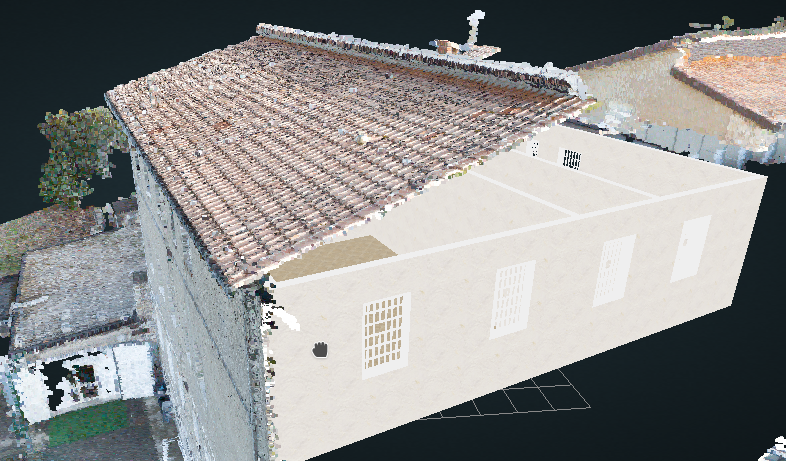
\includegraphics[width=1\linewidth]{images/augmented}
   \caption{A model inside a point cloud}
   \label{fig:augmented}
\end{figure}

\subsection{Risultati finali}

\noindent Terminate le fasi del workflow e validata la geometria del modello, l'applicazione fornisce una stima del costo di demolizione. Questo rappresenta l'output desiderato dall'utente in quanto permette di capire se le decisione prese sono corrette o conveniente dal punto di vista economico ed ambientale. Questo report finale si compone da quattro documenti:
\begin{itemize}
 \item Una stima dei volumi dei materiali di ogni singolo componente, ricavata a partire dalle geometrie definite in fase di modellazione con opportuni calcoli di integrazione.
 \item Una stima dei costi di demolizione, smaltimento e recupero. Partendo dai volumi, si determinano le masse grazie alle propriet\`a dei materiali, mentre conoscendo i CER e quindi la modalit\`a di smaltimento, si stimano i costi del conferimento in discarica.
 \item Una stima dei costi di trasporto necessari per trasferire i materiali dal sito di demolizione alla discarica. Per fare questo si tiene conto della posizione geografica del modello calcolando i percorsi stradali pi\`u convenienti.
 \item Un stima dei tempi previsti per la demolizione completa del fabbricato, collocati su un diagramma di Gantt. Per fare questo si utilizza l'informazione del cronoprogramma attribuito durante la fase di attribuzione della semantica.

\end{itemize}


\noindent